 \documentclass[11pt]{book}
 \usepackage{mystyle}

\begin{document}

%% GENERAL FORM

\section*{Introduction}

In this chapter we will devleop the mathmatical model for the dynamic
loudspeaker mechanical system.  Our goal is to predict the time response
of the system to an inital displacement or velocity.  This reveals
several key properties of the system including its natural resonant
frequency and amplitude decay over time.

A real speaker is, of course, driven by some external power source to
reproduce acoutsic pressure.  By considering the system apart from its
driving conditions we can separate out the aspects which describe the
mechanical system in all cases.

First we make the analogy between the dynamic loudspeaker and a mass
on a spring.  This is an apt comparison because the underlying
mechanical elements are similar.  Cone motion is subject to a
restoring force from its compliant elements just as a spring provides
such a force.  Cone motion is also opposed by mechanical
losses due to friction and drag.  We find the same in the mass-spring
system. The cone mass provides an intertia which must be
overcome to produce motion just as in the mass-spring system.

Next we formalize the quantities and forces which describe the
mass-spring system and develop the underlying differential equation
that they imply.  Constituent forces are added one at a time.  The
time response is analyzed at each step to show the effects of a
progressively more complex analysis.

Last we show that an equivalent electrical system may be determined,
which obeys the same differential equation.  This motivates our future
development of the analogous system circuit.



\section* {General equation}

The most general form of the harmonic oscillator is given by the
equation:

\begin{equation*}
  \Lambda_2 \ddot y + \Lambda_1 \dot y + \Lambda_0 y = \Gamma(t)
\end{equation*}

It is important to note that each derivative of the dependant variable
is multiplied by a constant and that the source term $\Gamma(t)$ can
be interpreted as an external force on the system.  When
$\Gamma(t) = 0$ the equation is termed 'homogenous.'

In mechanics this equation may represent the displacement of a mass
whose motion is subject to a restoring force proportional to its
displacement.  The simplest of which is a mass on a spring.


\section* {The free oscillator}

For such a system Hooke's Law gives:

%% Form1: no damping or driving
\begin{equation*}
  F = -kx 
\end{equation*}

where $k$ is the so-called spring constant.  Since, by Newton $F = ma$, this is

\begin{equation}
  \label{free_oscillator_system_equation}
  m \ddot x + kx = 0
\end{equation}

A solution to this equation is easy to determine by intuition.  We
require a solution $x$ which is proportional to its second
derivative.  This limits our choices considerably.  The sine and
cosine functions come to mind.

We will proceed by formal application of differential equations theory
to see if our intuition is supported.

\begin{equation}
  \label{free_oscillator_solution}
  x = Ae^{\alpha t}
\end{equation}

and it's derivatives

\begin{equation}
  \dot x = \alpha x \quad \quad  \ddot x = \alpha ^2 x
\end{equation}

plugging back into equation \eqref{free_oscillator_system_equation}
and dividing through by mass

\begin{equation*}
  \alpha^2 mx + kx = 0
\end{equation*}

from which the $\alpha$ is determined to be

\begin{equation*}
  \alpha = \pm j \sqrt{\frac{k}{m}} = \pm j \omega_o
\end{equation*}

where we recognize that $\alpha$ must assume the units of frequency to
keep our exponential argument unitless as requried.  Returnig to the
solution \eqref{free_oscillator_solution}

\begin{equation*}
  x = A_1e^{j\omega_o t} + A_2e^{-j\omega_o t}
\end{equation*}

By application of Euler's identity this can be rewritten in terms of
the sine and cosine functions as

\begin{equation*}
  x = A_1[cos(\omega_o t) + j sin(\omega_o t)] + A_2[cos(\omega_o t) - j sin(\omega_o t)]
\end{equation*}

Combining terms and renaming constants gives

\begin{equation*}
  x = B_1cos(\omega_o t) + B_2sin(\omega_o t)
\end{equation*}

Where $B_1$ and $B_2$ may be complex if necessary, and are determined
by inital conditions.

It is aparent then that the system resonates at frequency $\omega_o$
with constant amplitude for all time.  Though this fits intution
regards to its sinusoidal motion, we must admit that real mass-springs
systems to not go on for eternity with the same amplitude.  Our model
must be refined to take mechanical damping into account.

\section* {The damped oscillator}  

We assume that, in addition to the restoring force, the system
experiences a damping force proportional to its velocity
$F_{damp} = -b\dot x$ yielding the system equation:

%% Form2: with damping no driving
\begin{equation*}
  F = -kx -b \dot x
\end{equation*}

or

\begin{equation}
  \label{damped_oscillator_system_equation}
  m \ddot x + b \dot x + kx = 0
\end{equation}

A suitable solution may be suggested either by intuition or by basic
knowledge of differential equations.  Since we might guess that the
harmonic displacement should decay over time we might choose a
solution like \eqref{free_oscillator_solution} and add an exponentially
decaying term. This is indeed correct for a certain sub-class of
solutions.It would not, however, include systems with high mechanical
damping, a door damper, for instance.


Instead we will take our cue from differential equations theory and try

\begin{equation}
  \label{damped_oscillator_solution}
  x = A e^{\alpha t}
\end{equation}

and its derivatives

\begin{equation*}
  \dot x = \alpha x \quad \quad  \ddot x = \alpha^2x
\end{equation*}

going back to the system equation \eqref{damped_oscillator_system_equation}

\begin{equation*}
  m \alpha^2 x + b \alpha x + k x = 0
\end{equation*}

dividing through by $x$ and $m$ gives the system characteristic
equation

\begin{equation*}
  \alpha^2 + \frac{b}{m} \alpha + \frac{k}{m} = 0;
\end{equation*}

here we pause to take a result from above by noting
$\frac{k}{m} = \omega_o^2$ and proceed with the quadratic equation to
find the roots of $\alpha$

\begin{equation}
  \label{oscillator_roots}
  \alpha = -\frac{b}{2m} \pm \sqrt{\left(\frac{b}{2m}\right)^2 - \omega_o^2}
\end{equation}

we may save some space by assigning $\gamma = \frac{b}{2m}$ giving

\begin{equation*}
  \alpha = -\gamma \pm \sqrt{\gamma^2 - \omega_o^2}
\end{equation*}

now returning to the proposed solution
\eqref{damped_oscillator_solution}
gives the linear combination

\begin{equation*}
  x = A_1e^{t\left(-\gamma + \sqrt{\gamma^2 - \omega_o^2}\right)} + A_2e^{t\left(-\gamma - \sqrt{\gamma^2 - \omega_o^2}\right)}
\end{equation*}

We must now understand this equation in physical terms.  The
interpretation of the solution $x$ hinges upon the difference term
beneath the square root.  As we shall see three cases become aparent,
these are


    \begin{align*}
      \gamma^2 - \omega_o^2 &> 0 \text{\quad} \Rightarrow \text{\quad Overdamped system}\\
      \gamma^2 - \omega_o^2 &< 0 \text{\quad} \Rightarrow \text{\quad Underdamped system}\\
      \gamma^2 - \omega_o^2 &= 0 \text{\quad} \Rightarrow \text{\quad Critically damped system}
    \end{align*}
    
\subsection*{Overdamped}

In the case of an overdamped system we can see that the radical
expression must be positive.  Further

\begin{equation*}
  -\gamma \pm \sqrt{\gamma^2 - \omega_o^2} < 0
\end{equation*}

from which we can see that both terms of our solution contain a
decaying exponential term, the addition of which comprises the whole
solution.

\begin{equation*}
  x = A_1e^{-t(-\gamma + \sqrt{\gamma^2 - \omega_o^2})}  + A_2e^{-t(-\gamma - \sqrt{\gamma^2 - \omega_o^2})}
\end{equation*}

Qualitativley the response decays towards
zero with increasing time.  No oscillation occurs, hence the term
'overdamped.' Figure \ref{harmonic_oscillator_plots} shows a typical over
damped response.


\subsection* {Underdamped}

In contrast the underdamped scenario takes a different form.  Here the
radical term must be negative.  It is helpful to rewrite the roots of
$\alpha$ in the following way

\begin{equation*}
  \alpha = -\gamma \pm i\sqrt{\omega_o^2 - \gamma^2}
\end{equation*}

The units of $\alpha$ must be that of angular frequency to keep the
exponential argument in our solution unitless.  From this we can also
see that $\gamma$ must, likewise, have units of angular frequency.

With this fact in hand we may interpret the radical term as a
modification of the natural resonant frequency due to damping.  The
damped resonant frequency can then be expressed as

\begin{equation*}
  \omega_d = \sqrt{\omega_o^2 - \gamma^2}
\end{equation*}
Which leads to a more compact and intuitve form of the solution

\begin{equation*}
  x = A_1e^{t(-\gamma + i\omega_d)} + A_2e^{t(-\gamma - i\omega_d)}
\end{equation*}

and may be broken down further to

\begin{equation*}
  x = e^{-\gamma t}(A_1e^{i \omega_d t} + A_2e^{ - i \omega_d t})
\end{equation*}

each term containing a decaying exponential and a complex exponential.
To interpret the complex exponential terms we employ Euler's equation
to find

\begin{equation*}
  x = e^{-\gamma t}(A_1[cos(\omega_d t) + i sin(\omega_d t)] + A_2[cos(\omega_d t) - i sin(\omega_d t)])
\end{equation*}

combining terms

\begin{equation*}
  x = e^{-\gamma t}([A_1 + A_2][cos(\omega_d t)] + i [A_1 - A_2][sin(\omega_d t)])
\end{equation*}

The addition or subtraction of the arbitrary constants may be combined
under new labels.  Also the $i$ factor may be absorbed into our chosen
constants as no real-valued restriction has been placed upon them.
This gives

\begin{equation*}
  x = e^{- \gamma t}(B_1cos(\omega_d t) + B_2sin(\omega_d t))
\end{equation*}

Finally sinusoidal terms of the same argument may be combined by a
well known trigonometric identitiy resulting in

\begin{equation*}
  x = Be^{- \gamma t}sin(\omega_d t + \phi)
\end{equation*}

As required the second order system has resulted in a solution with
two unknowns,
namely $B$ and $\phi$, which may be determined by initial conditions.

Importantly we note that our solution now has a clear physical
interpretation.  We expect oscillation with the damped frequency of
$\omega_d$ which decays over time to zero owing to its leading
exponential term.
\subsection*{Critically Damped}

The last scenario to consider is when the radical expression is
exactly zero.  In real systems this is never strictly achieveable but
serves as a singluar transition state between the over and underdamped
scenarios.  It is worth
taking the time to describe its behavior.

Straight away we see that our expression for $\alpha$ in
\eqref{oscillator_roots} produces only
one root and hence our solution is no longer a linear combination with
the required two constants.  By basic differential equations theory or
by direct computation we can see that another solution may be
proposed, namely

\begin{equation*}
  x = tAe^{\alpha t}
\end{equation*}

leading to the entire solution

\begin{equation*}
  x = A_1e^{\gamma t} + t A_2e^{\gamma t}
\end{equation*}

where $\gamma$ is as defined above. Qualitatively this solution is similar to the overdamped case.
However it represents the fastest possible decay towards zero without
oscillation.  Any higher damping would lead to a slower approach, any
lower damping would lead to undershooting zero and oscillatory
behavior.  Figure \ref{harmonic_oscillator_plots} shows one such
critically damped response.

\begin{figure}[h!]

  \centering
  \frame{
    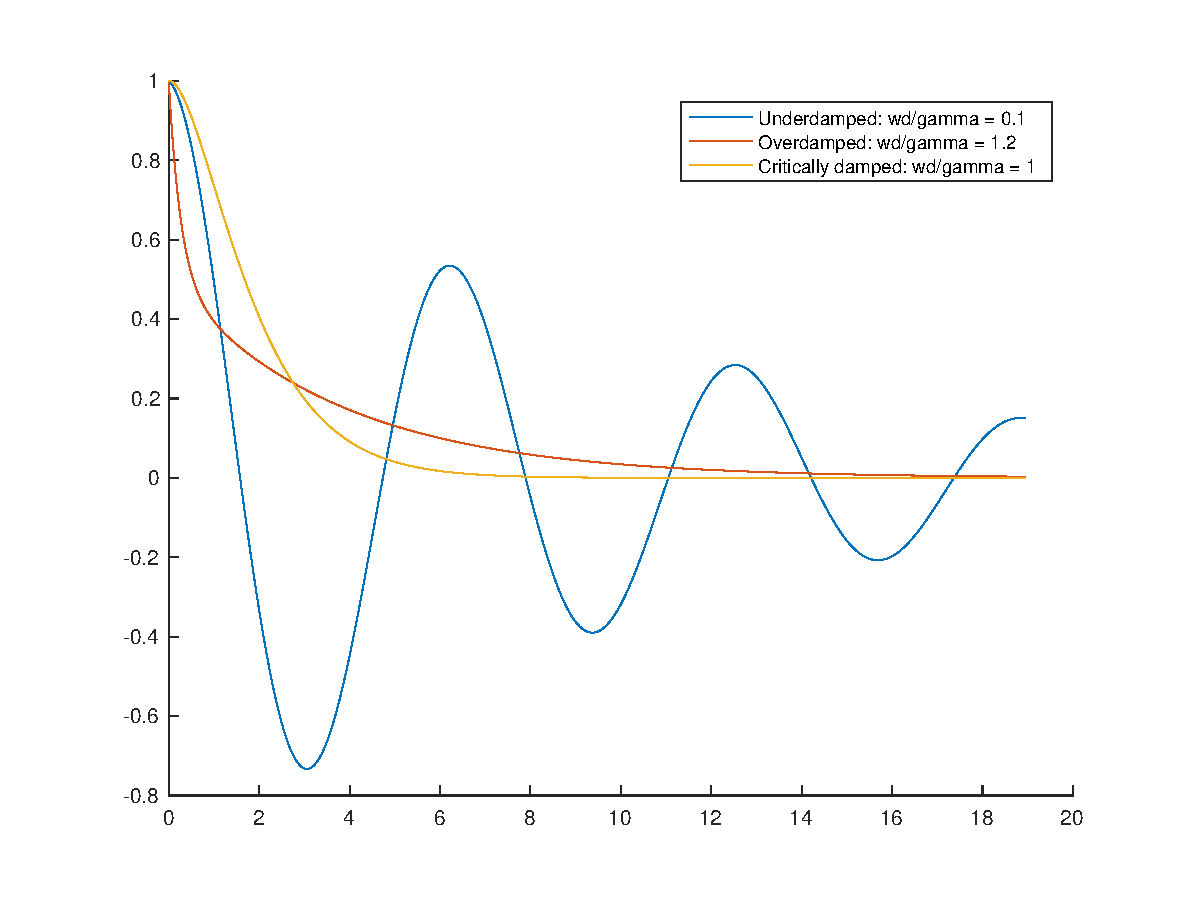
\includegraphics[width=\linewidth]{./img/SHO_plots.eps}
    }
    \caption{Under, Over, and Critically damped system response}
      \label{harmonic_oscillator_plots}
\end{figure}

\section*{General equation revisited}
Having come this far we now look back on the results obtained in light
of the general equation of harmonic motion.

In terms of constants given we can generalize the behavior of any
system obeying this fundamental differential equation.  Following the
development above such a system has the characteristic equation

\begin{equation*}
  \alpha^2 \Lambda_2 + \alpha \Lambda_1 + \Lambda_0 = 0
\end{equation*}

whose roots are
\begin{equation*}
\alpha = \frac{\Lambda_1}{2\Lambda_2} \pm \sqrt{\left(\frac{\Lambda_1}{2\Lambda_2}\right)^2 + \left(\frac{\Lambda_0}{\Lambda_2}\right)}  
\end{equation*}

the solutions to the free, overdamped, underdamped, and critically
damped scenarios are formally equivalent to those already given.  In terms of
our generalized constants the system exhibits the following characteristics

a natural resonant frequency of

\begin{equation*}
  \omega_o = \sqrt{\frac{\Lambda_0}{\Lambda_2}}
\end{equation*}

an exponential decay argument including

\begin{equation*}
  \gamma = \frac{\Lambda_1}{2\Lambda_2}
\end{equation*}

and a damped resonant frequency of

\begin{equation*}
  \omega_d = \sqrt{\omega_o^2 - \gamma^2}
\end{equation*}

Where damping is absent $\Lambda_1 = 0$ hence $\gamma = 0$ and no
decay occurs.  Where damping is present the
value of $\gamma^2 - \omega_o^2$ 
determines the classification as underdamped, overdamped, or
critically damped

Hence any system sharing the same governing differential equation may be
immediately solved by considering only its constants.


\section*{The series L-C-R circuit}

\begin{figure}[h!]
  \centering
    \begin{circuitikz}[scale=1.3]
      \draw (0,0)
      to[short](0,2)
      to[R=$R$] (2,2)
      to[L=$L$] (4,2)
      to[C=$C$] (6,2)
      to[short] (6,0)
      to[short] (0,0);
    \end{circuitikz}
   \caption{Sourceless series L-C-R circuit}
  \end{figure}

  
  From basic circuit theory we understand the current and voltage
  behavior of the usual passive elements to be:

  
  Resistors, by ohms law

  \begin{equation*}
    e = iR
  \end{equation*}

  Inductors

  \begin{equation*}
    e = L \frac{di}{dt} \text{\qquad and \qquad} i = \frac{1}{L} \int e \,dt
  \end{equation*}

  Capacitors

  \begin{equation*}
     e = \frac{1}{C}\int i \,dt  \text{\qquad and \qquad} i = C\frac{de}{dt}
   \end{equation*}

   where $e$ and $i$ are voltage and current and $L$, $C$, and $R$
   denote inductance, capacitance, and resistance respectively.

   From these a system equation for the series LCR circuit may be
   written.  In particular we assign sum of the component voltage
   drops to be zero since there is no source, giving

   \begin{equation*}
     L \frac{di}{dt} + iR + \frac{1}{C} \int i \,dt = 0
   \end{equation*}

   Taking the time derivative of both sides yields

   \begin{equation*}
     L\frac{d^2i}{dt^2} + R\frac{di}{dt} + \frac{1}{C}i = 0
   \end{equation*}

   We have arrived again at the familiar form of the harmonic
   oscillator.  Drawing parallels to our mechanical analysis of the
   mass-spring system we can see:

   \begin{align*}
     \Lambda_2 &\Rightarrow \text{Mass} \Rightarrow \text{Inductance}\\
     \Lambda_1 &\Rightarrow \text{Damping Constant} \Rightarrow \text{Resistance}\\
     \Lambda_0 &\Rightarrow \text{Spring Constant} \Rightarrow \text{1/Capacitance}\\
   \end{align*}

   The solutions of the LCR system current must, then, take identical
   forms to those of displacement in the mass-spring system.  Further,
   and perhaps less obviously, the mass-spring system may be
   represented as a series LCR circuit if care is taken to map each parameter to
   its corresponding circuit element.

   This translation into circuit form is known as lumped parameter
   modeling.  It provides insight by availing us of the many tools and
   techniques used for circuit analysis.
   
   
  

\end {document}


%%% Local Variables:
%%% mode: latex
%%% TeX-master: t
%%% End:
